\section{Datasets}
    \todo{write about the datasets show images}
    
    \subsection{kvasir}


    Automatic computerised detection of diseases has been an essential focus on the medical industry, but for a long time, a still fairly unexplored research area.  As a response to this Simula Research laboratory together with \todo{more}, made the dataset Kvasir.
    It was originally made to improve medical practice and refine health care systems where similar dataset did not exist.

    Kvasir is a dataset containing images from inside the gastrointestinal tract containing three anatomical landmarks, in the form of (A), (B) and (C). Also, the Kvasir dataset includes two categories of images related to endoscopic polyp removal, (D) and (E). And lastly, three classes, (G), (H), and (I), containing images without the anomalies, as a form of baseline. 
    Medical professionals sorted the dataset, and it is made to be used for both single and multi-disease computer-aided detection. 


    At this time, there are two versions of the kvasir dataset.  V1 vs V2
    The images are from both from the lower and upper GI tract, 
    Talk about the classes. 
    Talk about the overlays.  
    
    
    
    %\textbf{The human digestive system may be affected by several diseases. Altogether esophageal, stomach and colorectal cancer accounts for about 2.8 million new cases and 1.8 million deaths per year. Endoscopic examinations are the gold standards for investigation of the GI tract. Gastroscopy is an examination of the upper GI tract including esophagus, stomach and first part of small bowel, while colonoscopy covers the large bowel (colon) and rectum. Both these examinations are real-time video examinations of the inside of the GI tract by use of digital high definition endoscopes. Endoscopic examinations are resource demanding and requires both expensive technical equipment and trained personnel. For colorectal cancer prevention, endoscopic detection and removal of possible precancerous lesions are essential. Adenoma detection is therefore considered to be an important quality indicator in colorectal cancer screening. However, the ability to detect adenomas varies between doctors, and this may eventually affect the individuals’ risk of getting colorectal cancer. Endoscopic assessment of severity and sub-classification of different findings may also vary from one doctor to another. Accurate grading of diseases are important since it may influence decision-making on treatment and follow-up. For example, the degree of inflammation directly affects the choice of therapy in inflammatory bowel diseases (IBD). An objective and automated scoring system would therefore be highly welcomed. Automatic detection, recognition and assessment of pathological findings will probably contribute to reduce inequalities, improve quality and optimize use of scarce medical resources. Furthermore, since endoscopic examinations are real-time investigations, both normal and abnormal findings have to be recorded and documented within written reports. Automatic report generation would proba- bly contribute to reduce doctors’ time required for paperwork and thereby increase time to patient care. Reliable and careful docu- mentation with the use of minimal standard terminology (MST) may also contribute to improved patient follow-up and treatment. To our knowledge, a standardized and automatic reporting system that ensure high quality endoscopy reports does not exist. In order to make the health care system more scalable and cost effective, basic research in the intersection between computer science and medicine must go beyond traditional medical imaging by combining this area with multimedia data analysis and retrieval, artificial intelligence, and distributed processing. Next-generation medical big-data applications are a frontier for innovation, compe- tition and productivity, where there are currently large initiatives both in the EU and the US. In the area of multimedia research, people are starting to see the synergies between multimedia and medical systems. For automatic algorithmic detection of abnormalities in the GI tract, there have been many proposals from various research communities, especially for the topic of polyp detection. However, the results are hard to reproduce due to lack of available medical data, i.e., the work listed above all use different and non-public data sets. Here, we therefore publish Kvasir: A Multi-Class Image Dataset for Computer Aided Gastrointestinal Disease Detection from the Vestre Viken Health Trust (Norway) containing not only polyps, but also two other findings, two classes related to polyp removal and three anatomical landmarks in the GI tract.}
    
    \newpage
    %============================================
    \begin{figure}[t]
        \centering
        \subfloat[\centering g]{
            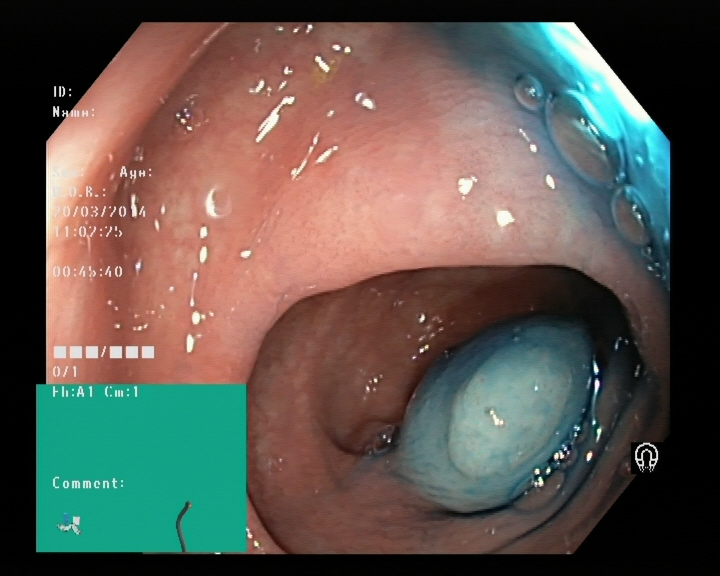
\includegraphics[width=4.5cm, height=4.5cm]{experiments/images/dyed-lifted-polyps.jpg}
        }
        \subfloat[\centering g]{
            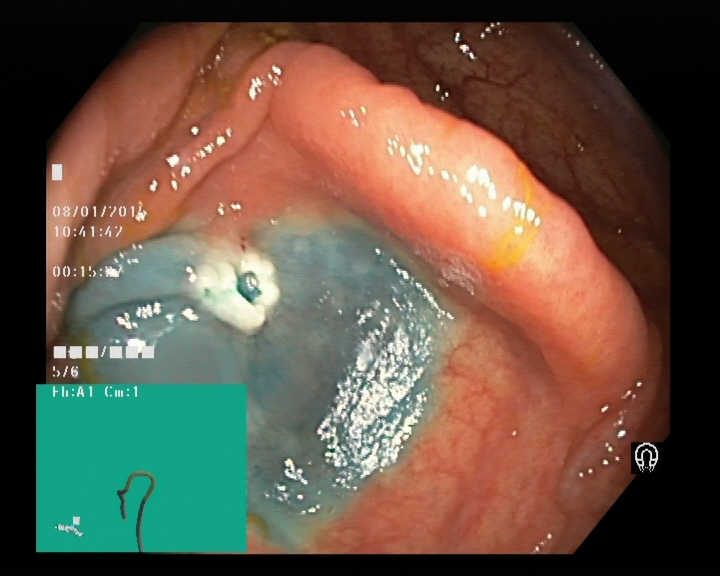
\includegraphics[width=4.5cm, height=4.5cm]{experiments/images/dyed-resection-margins.jpg}
        }
        \hspace{0mm}
        \subfloat[\centering g]{
            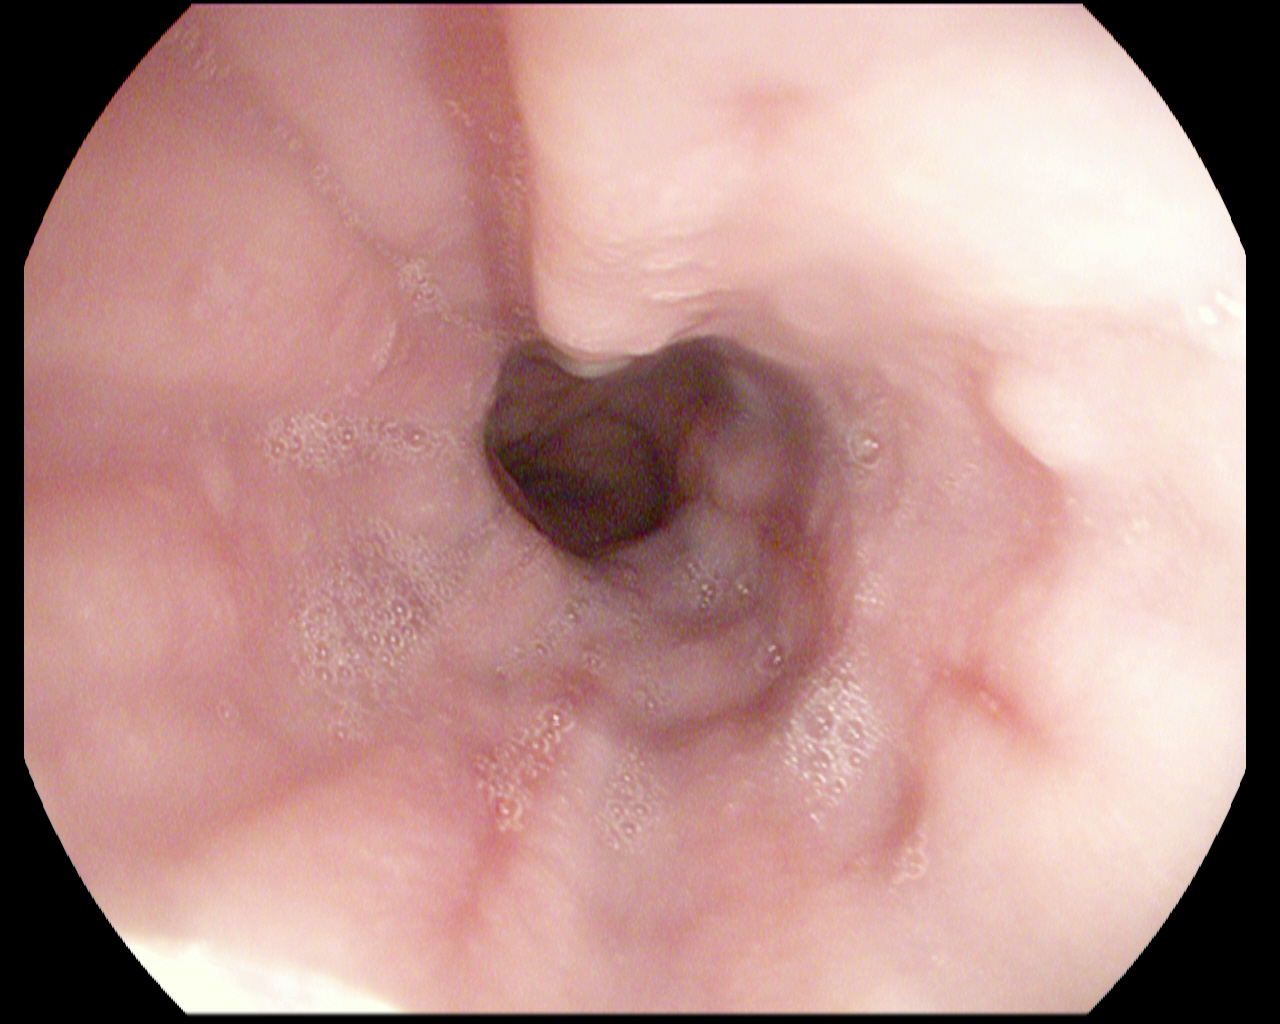
\includegraphics[width=4.5cm, height=4.5cm]{experiments/images/esophagitis.jpg}
        }
        \subfloat[\centering g]{
            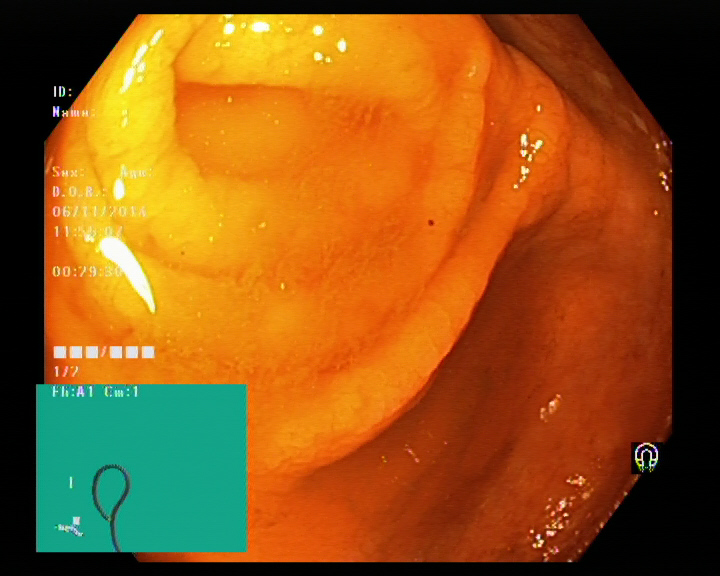
\includegraphics[width=4.5cm, height=4.5cm]{experiments/images/normal-cecum.jpg}
        }
        \hspace{0mm}
        \subfloat[\centering g]{
            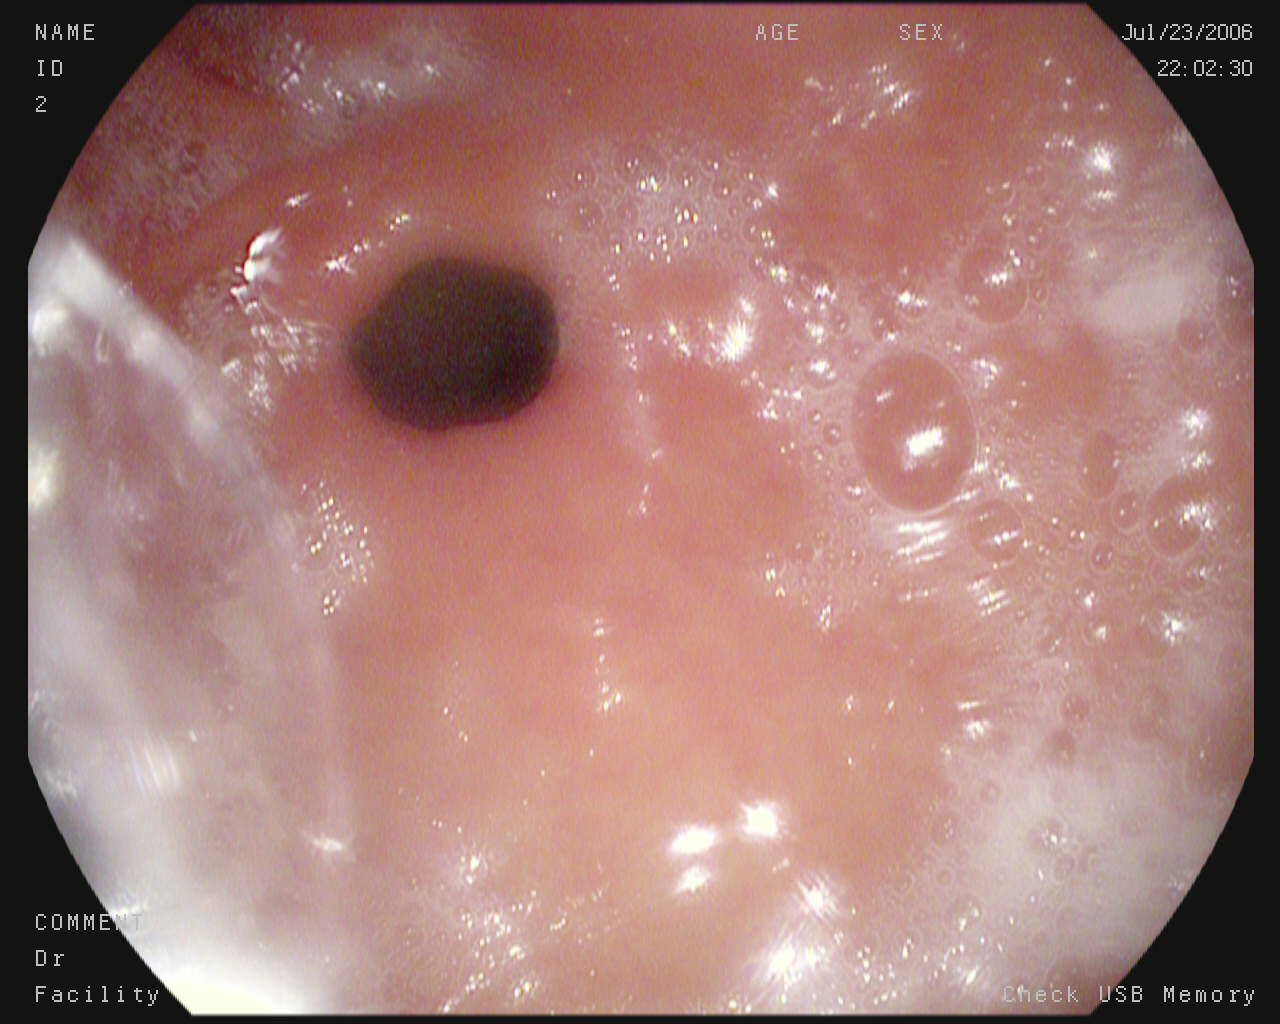
\includegraphics[width=4.5cm, height=4.5cm]{experiments/images/normal-pylorus.jpg}
        }
        \subfloat[][\centering g]{
            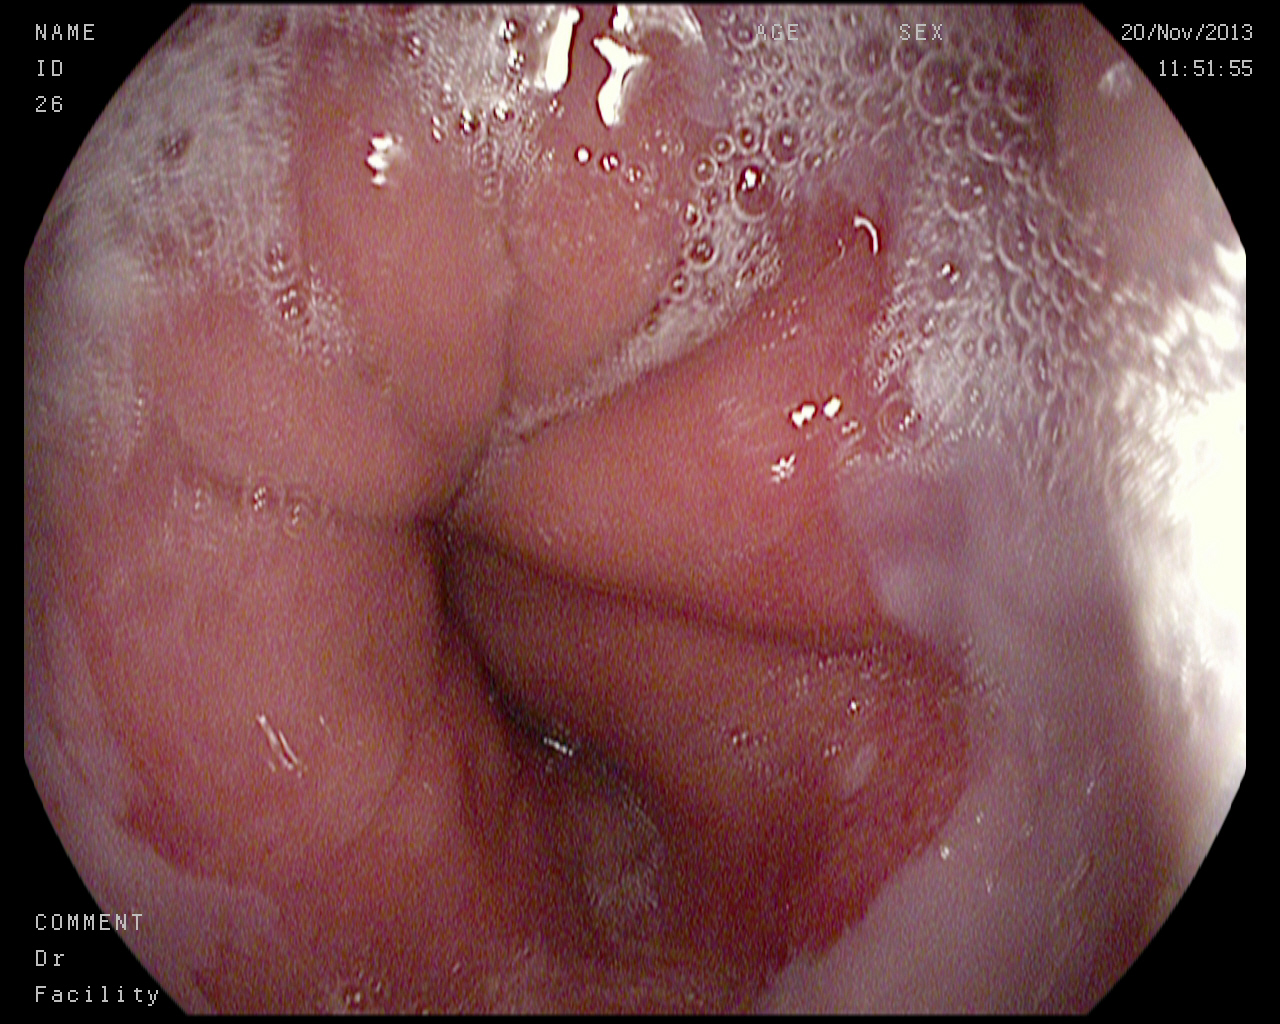
\includegraphics[width=4.5cm, height=4.5cm]{experiments/images/normal-z-line.jpg}
        }
        \hspace{0mm}
        \subfloat[\centering g]{
            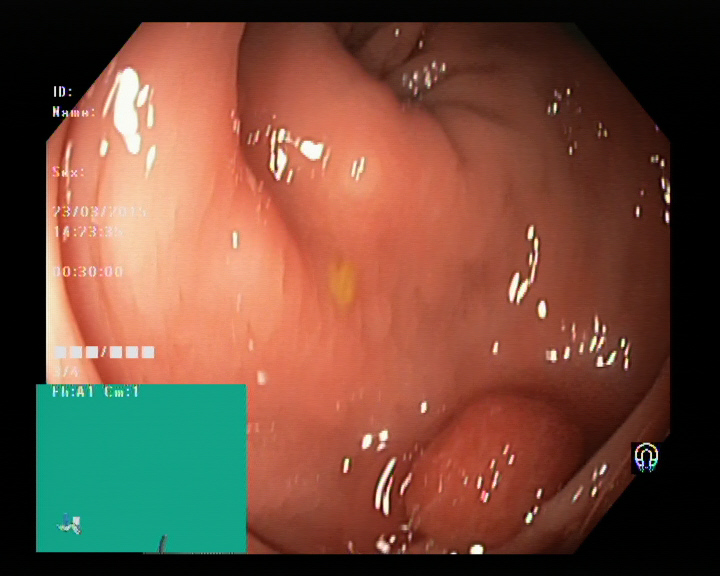
\includegraphics[width=4.5cm, height=4.5cm]{experiments/images/polyps.jpg}
        }
        \subfloat[\centering g]{
            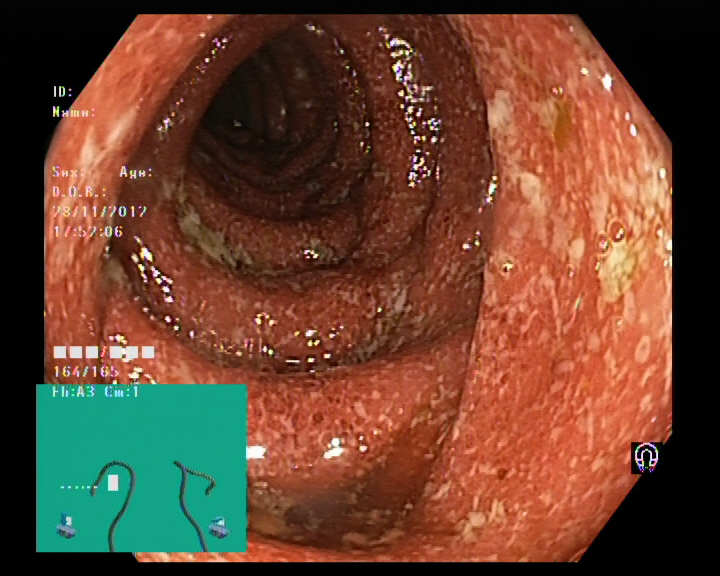
\includegraphics[width=4.5cm, height=4.5cm]{experiments/images/ulcerative-colitis.jpg}
        }
        \caption{Same image from the z-line with four different inpainting attempts. Each image is re-sized to fit in the figure.}
        \label{fig:images_16}
    \end{figure}
    %=============================================
    \subsection{CVC-356}
    \subsection{CVC-12k}
    \subsection{CVC-612}

\section{Metrics}
When we are measuring preprocessing and classifying, we need a metric to evaluate. In some cases, we want to maximise similarity, and other times minimise error. 
For the preprocessing, the associated metric can be the mean square error (MSE), \todo{more}

For the transferlerning, the associated metric can either be Validation accuracy or validation loss. 
Validation accuracy is a number between 0% and 100%, where our goal is to get the latter.
At 100% we classify every sample correct, \todo{more}.

Validation loss is a measure of how well the training is doing at a given time \todo{We have maybe talked about this earlier}. The goal for the loss is to reach the value 0, and it can be arbitrarily high.

\subsection{Common metrics}
List:
Taken from Kvasir site\todo{cite}

True positive (TP)    The number of correctly identified samples. The number of frames with an endoscopic finding which correctly is identified as a frame with an endoscopic finding.

True negative (TN)    The number of correctly identified negative samples, i.e., frames without an endoscopic finding which correctly is identified as a frame without an endoscopic finding.

False positive (FP)    The number of wrongly identified samples, i.e., a commonly called a "false alarm". Frames without an endoscopic finding which is erroneously identified as a frame with an endoscopic finding.

False negative (FN)    The number of wrongly identified negative samples. Frames without an endoscopic finding which erroneously is identified as a frame with an endoscopic finding.

Recall (REC)    This metric is also frequently called sensitivity, probability of detection and true positive rate, and it is the ratio of samples that are correctly identified as positive among all existing positive samples.

Precision (PREC)    This metric is also frequently called the positive predictive value, and shows the ratio of samples that are correctly identified as positive among the returned samples (the fraction of retrieved samples that are relevant).

Specificity (SPEC)    This metric is frequently called the true negative rate, and shows the ratio of negatives that are correctly identified as such (e.g., the fraction of frames without an endoscopic finding are correctly identified as a negative result).

Accuracy (ACC)    The percentage of correctly identified true and false samples.

Matthews correlation coefficient (MCC)    MCC takes into account true and false positives and negatives, and is a balanced measure even if the classes are of very different sizes.

F1 score (F1)    A measure of a test’s accuracy by calculating the harmonic mean of the precision and recall.

\subsection{Singleclass vs Multiclass Metrics}

The metrics presented are, in general, a solid way to present the validity of a model. However, not all metrics presented is the same when switching between single and multiclass classification.  Metrics like Accuracy is designed to work for multiclass classification, given that there is only one way to calculate the score.
\begin{equation}
        \frac{sum(diag(covariance_matrix))}{sum(covariance_matrix))}
\end{equation}
	
	


The problem with multiclass metrics is more significant in the case for instance Recall and Specificity, where we have multiple ways to calculate the score. 
We have chosen in this paper to focus on the \todo{Weighted} average of our Multiclass metrics. 

In addition to looking at the weighted average of precision and recall, we want to look at specific cases of the classification.  In many cases, we have multiple classes, where we are most interested in just one or a handful of the classes shown. 
For instance, a focus we have in this theis is to give a score on how predictable polyp detection is, and on that case, we want to discuss the True positive rate (TPR) of the polyp detection and not the TPR of the non-polyp classes. 

Take for instance the matrix shown in \todo{fig}\\
\begin{verbatim}
    [[10 1]
     [3 12]]
\end{verbatim}

 Here we can calculate the weighted average recall to be \textbf{x}. This can be an interesting observation in itself, but often the first or second True label is much more important relative to the other.  In a more practical example: We are more interested in finding areas with polyps when we know they are present, compared knowing there are not a polyp in an area when none are present. 

These Metrics becomes a more prominent topic when it comes to inpainting. With inpainting, we take areas with no relevant information and makes it into areas that are similar to the rest of the image. Given that we can inpaint over polyps by mistake, or that we might train our classifiers to not look in certain areas when classifying, we have an interest if also comparing single cases of recall and precision included to the average values.

    \section{Setup of experiments}



\section{format of experiments}
    \subsection{Inpaint}
    \subsection{Classifying}
    
\section{Inpainting Kvasir}
    \subsection{Black corners}
    \subsection{Green square}
    \subsection{Text}
    \subsection{Combination}
    \subsection{Random masking}
    
\section{Kvasir -> CVC612}
\section{Kvasir -> CVC 12k}
\section{Kvasir -> CVC356}

\section{Summary
}
